\documentclass[12pt, a4paper]{mwart}

\usepackage[utf8]{inputenc}								%kodowanie znaków
\usepackage[T1]{fontenc}									%kodowanie fontu
\usepackage{polski}										%polskie wcięcia itp
\usepackage{graphicx}									%wstawianie grafik
\usepackage{enumitem}									%lista a), b), c)
\usepackage{courier}										%Courier New w tekście
\usepackage{listings}									%kod źródłowy
\usepackage{amsmath}
\usepackage{xcolor}

\linespread{1.3}											%interlinia 1,5
\usepackage[hidelinks]{hyperref}						%linki w spisie treści
\hypersetup{linktoc=all}

\lstset{
basicstyle=\scriptsize,
literate=%
{ą}{{\k{a}}}1
{Ą}{{\k{A}}}1
{ć}{{\'c}}1
{Ć}{{\'{C}}}1
{ę}{{\k{e}}}1
{Ę}{{\k{E}}}1
{ł}{{\l{}}}1
{Ł}{{\L{}}}1
{ń}{{\'n}}1
{Ń}{{\'N}}1
{ó}{{\'o}}1
{Ó}{{\'O}}1
{ś}{{\'s}}1
{Ś}{{\'S}}1
{ż}{{\.z}}1
{Ż}{{\.Z}}1
{ź}{{\'z}}1
{Ź}{{\'Z}}1
}

\begin{document}
\begin{center}
Piotr Wróbel\\
NLP \ppauza raport
\end{center}
  
\section{Wyniki treningu na dostarczonym zbiorze danych}

\subsection{Sieć neuronowa}

Output:
\begin{lstlisting}
INFO:simpletransformers.classification.classification_model:
{'mcc': 0.8984277314260114, 
 'tp': 119, 
 'tn': 124, 
 'fp': 7, 
 'fn': 6, 
 'acc': 0.94921875, 
 'eval_loss': 0.2754532750695944}
\end{lstlisting}

Stąd precyzja wynosi około 95\%.

\subsection{Klasyfikator Bayesowski}

\begin{figure}[ht]
  \centering
  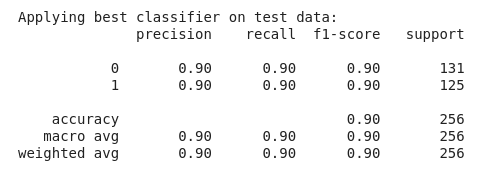
\includegraphics[width=0.7\textwidth]{images/bayes.png}
\end{figure}

\section{Modyfikacja hiper-parametrów}

Testowano zmiany liczby epok i~rozmiaru batcha, rozmiarów batcha mniejszych od 10 nie testowano, gdyż dla najwyższej użytej liczby epok (20) trenowanie modelu trwało zbyt długo.

\section{Własny zbiór danych}

Wybrano fragmenty pierwszego tomu ,,Ogniem i mieczem'' oraz ,,Odyseji'' z~tesktów dostępnych w~portalu wolnelektury.pl. Kryterium doboru tych pozycji były różne epoki w~jakich powstawały oraz fakt, że jedna z~nich jest tekstem oryginalnym a~druga tłumaczeniem. Ze względu na zbyt długi czas treningu modelu dla całego tekstu, z~każdego z~nich wyciągnięto po 1000 zdań rozpoczynając od 50 z~kolei (aby pominąć numery ISBN, tytuł i~inne nieistotne w~tym ćwiczeniu informacje zamieszczane na początku utworu). Zbiór danych jest dostępny pod adresem: \url{https://github.com/pwrobel5/msi/blob/master/nlp/text_set.csv}

\section{Wyniki treningu modelu dla własnego zbioru danych}

Zastosowano liczbę epok równą~5 i~domyślny rozmiar batcha (8).

\end{document}